POSIX provides three main types of IPC: streams, datagrams and shared memory.  
A review of each is made before making a choice for desired message passing skeam.

\noindent \textbf{Streams:}\\
The IPC type \textit{stream} includes pipes, FIFOs, stream sockets, and TCP sockets.
All stream basted methods suffer from head of line (HOL) blocking which means older data \textbf{must} be read before newer data.
%In addition all streaming methods are exposed to file abstraction (read/write byte sequence).
For robotic applications we must be able to access the newest data imediately and read older data if needed.
This is a different paradime then typical streaming application because robots are real-time sensitive meaning the newest information holds more value to the overall system than the older data.

\noindent \textbf{Datagrams:}\\
POSIX \textit{datagrams} come in two major flavors, \textit{datagram sockets} and \textit{POSIX message queues}.
Datagram sockets are less likely to block the sender then streams.
The most important reason why datagrams are \textbf{not} a good solution for my application is that newer messages are lost if the buffer is filled.
Newer data is more important than older data in my control system thus this is not a viable option.

POSIX message queues are simular to datagrams sockets with the addition of message priorities.
Unlike datagram sockets if the buffer fills the POSIX message queues will block.
This will cause the application to stop processing until it is able to read/flush the old messages.
Thus simular to other methods mentioned this also suffers from HOL.

\noindent \textbf{Shared Memory:}\\
POSIX shared memory is very fast and allows access to the latest data by simply writing over a variable.
Though I have been advicating that the newest information is the most important, old information can not be discarded.
If using POSIX shared memory there is no way of recovering older data that might have been missed by a controller.

What is needed is a method of sharing data that is \textit{non-blocking} and as \textit{low-latancy} like shared memory, but still holds older data and uses an asyncronous IO scheme.
The asyncronous IO scheme is required so the controller is not locked to a set rate by the data transactionn method.
N. Dantam et. al.\cite{ach} shows that Asynchronous IO (AIO) might be approperiate for this application however the implimentaiton under Linux is not as mature as I require.
In addition N. Dantam shows that other IPC mechanism using select/poll/epoll/kqueue are widely used network server and help midigate but not totally removed the issue of HOL.
The primary problem being that that thought the sender will not block the reader must stil read the oldest data first.
The question now is what IPC mechanism will be suitable for my control system.



\begin{figure}[thpb]
  \centering
      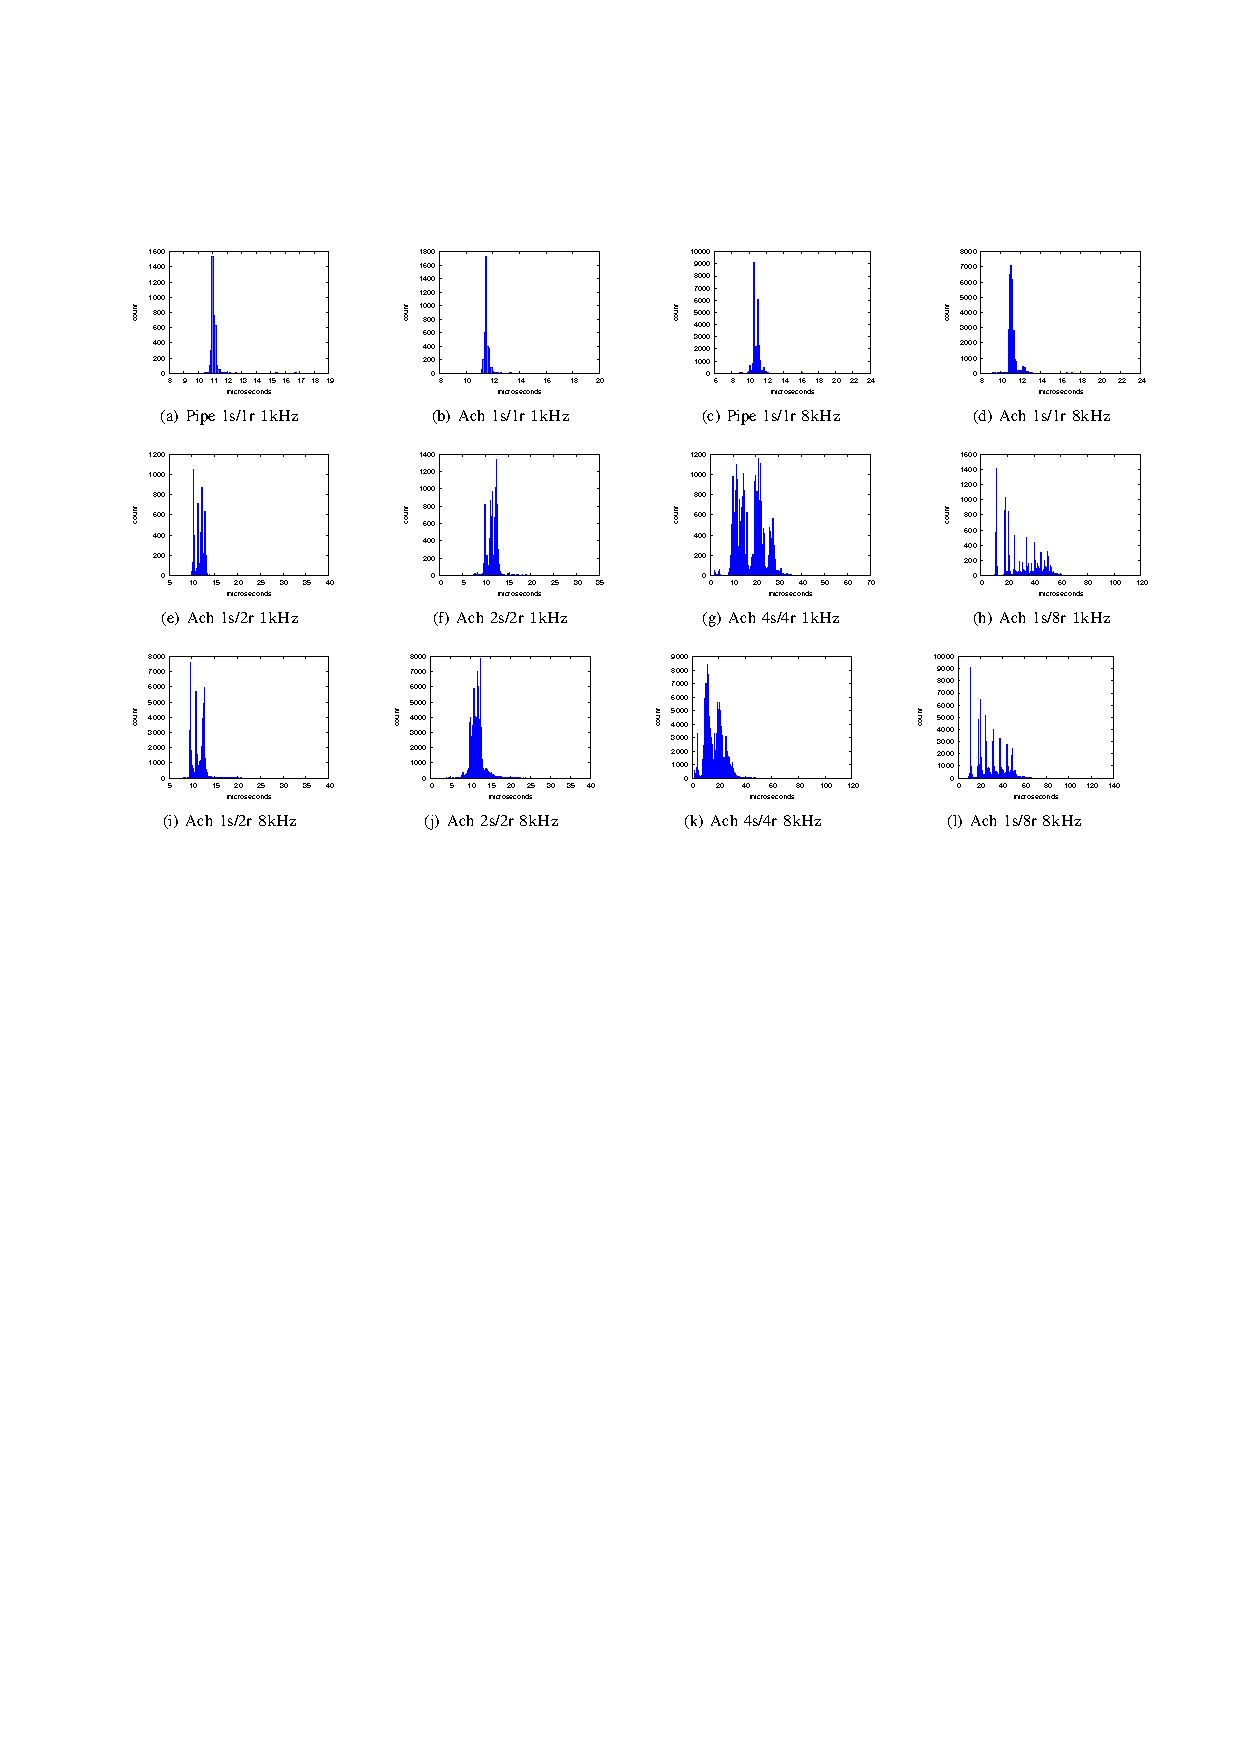
\includegraphics[width=1.0\columnwidth]{./hubo-ach/pix/dantam2012robustAchTiming.pdf}\\
\caption{Histograms of Ach and Pipe messaging latencies. Benchmarking performed on a Core 2 Duo running Ubuntu Linux 10.04 with PREEMPT
kernel. The labels $\alpha$s/$\beta$r indicate a test run with $\alpha$ sending processes and $\beta$ receiving processes\cite{ach}.}
\label{fig:ach-timing}
\end{figure}




Upon investigation three major mechanisms are avaliable; Robot Operating System (ROS)\cite{ros}, Message Passing Interface (MPI)\cite{Gropp:1999:UMP:330577} and Ach\cite{ach}.
Though ROS is ubicuitious in the robotics and automation field the inherent latency and the non real-time (RT) guarantee due to the use of TCP/IP it is not a good choice.
MPI is ubiquitous in the high-proformance computing field.  It has full non-blocking capiabilities and is geared towards maximizing message throughput for networked clusters\cite{ach}.
Table~\ref{table:ipc} shows a comparision of a wide range of IPC methods.
A focus on reducing latency is not given.
Ach does focuses on latency.
Fig.~\ref{fig:ach-timing} shows histograms of Ach and Pipe messaging latencies. Benchmarking performed on a Core 2 Duo running Ubuntu Linux 10.04 with PREEMPT
kernel. The labels $\alpha$s/$\beta$r indicate a test run with $\alpha$ sending processes and $\beta$ receiving processes.

\begin{table}
\caption{Robot control system comparison}
\begin{tabular}{l || c | c | c | c | c | c}
\hline
System                          & Open        & POSIX           & Non          & Real      & Low         & Light \\
                                &      Source &       Complaint &     Blocking &      Time &     Latency & Weight\\
\hline
\hline
ROS                             & yes         & yes             & no           & no        & no          & no \\
\hline
Orocos Real-Time                & yes         & yes             & no           & yes       & yes         & no \\
                 Toolkit        &             &                 &              &           &             &    \\
\hline

Robotics Technology             & yes         & yes             & no           & yes       & yes         & no \\
                    Middleware  &             &                 &              &           &             &    \\
\hline
Microsoft Robotics              & no          & no              & no           & yes       & yes         & no \\
                   Studio       &             &                 &              &           &             &    \\
\hline
Aware2.0                        & no          & yes             & no           & yes       & yes         & yes \\
\hline
Hubo-Ach                        & yes         & yes             & yes          & yes       & yes         & yes \\



\hline
\end{tabular}
\label{table:robotOS}
\end{table}


\begin{table}\label{table:ipc}
\caption{Inter Process Comunication Method Comparison}
\small
\begin{tabular}{l || c | c | c | c | c | c | c}
\hline
Inter-                          & Open        & POSIX           & Non          & Multiple    & Low         & Light   & Access \\
Process                         &      Source &       Complaint &     Blocking & Senders     &     Latency & Weight  & Old   \\
Comunication                    &             &                 &              & and         &             &         & Data          \\
Method                          &             &                 &              & Receivers   &             &         &           \\
\hline
\hline
Streams                         & yes         & yes             & no           & yes       & no          & yes     & yes \\
\hline
Datagram                        & yes         & yes             & no           & yes       & no          & yes     & yes \\
Sockets                         &             &                 &              &           &             &         &     \\
\hline

POSIX                           & yes         & yes             & no           & yes       & no          & yes     & yes\\
Message                         &             &                 &              &           &             &         &     \\
Queues                          &             &                 &              &           &             &         &     \\
\hline
Shared                          & yes         & yes             & yes          & yes       & yes         & yes     & no \\
Memory                          &             &                 &              &           &             &         &     \\

\hline
AIO                             & yes         & yes             & yes          & yes       & yes         & yes     & yes \\
\hline
CORBA                           & yes         & yes             & yes          & no        & yes         & yes     & yes \\
\hline
ROS                             & yes         & yes             & no           & yes       & no          & no      & no \\
\hline
Data                            & yes         & yes             & yes          & yes       & yes         & yes     & yes\\
Distribution                    &             &                 &              &           &             &         &     \\
Service                         &             &                 &              &           &             &         &     \\
\hline
Ach                             & yes         & yes             & yes          & yes       & yes         & yes     & yes\\


\hline
\end{tabular}
\normalsize
\end{table}

